\documentclass[a4paper,12pt,titlepage]{article}
\usepackage[utf8]{inputenc}
\usepackage[czech]{babel}
\usepackage{amsfonts, amsmath, amsthm, amssymb}
\usepackage[small,compact]{titlesec}
\usepackage{anyfontsize}
\usepackage{rotating}
\usepackage{mdwlist}
\usepackage[left=1.5cm,right=1.5cm,top=1.5cm,bottom=2cm]{geometry}
\usepackage{wrapfig}
\usepackage{subcaption}
\usepackage{hyperref}
\usepackage{color}
\usepackage{tikz}
\newcommand*\circled[1]{\tikz[baseline=(char.base)]{
  \node[shape=circle,draw,inner sep=1pt] (char) {#1};}}

\usepackage{titlesec}
\titleformat*{\section}{\removelastskip\bigskip\LARGE\bfseries}
\titleformat*{\subsection}{\large\bfseries}
\titleformat*{\subsubsection}{\large\bfseries}

\newcommand{\shn}{\Theta}
\newcommand{\lm}{\smallskip\noindent\bf Lemma\rm{} }
\newcommand{\dk}{\smallskip\noindent\bf Důkaz\rm{} }
\newcommand{\df}{\smallskip\noindent\bf Definice\rm{} }
\newcommand{\vt}{\smallskip\noindent\bf Věta\rm{} }
\newcommand{\poz}{\smallskip\noindent\bf Pozorování\rm{} }
\newcommand{\pzn}{\smallskip\noindent\bf Poznámka\rm{} }
\newcommand{\dsl}{\smallskip\noindent\bf Důsledek\rm{} }
\newcommand{\tv}{\smallskip\noindent\bf Tvrzení\rm{} }
\newcommand{\F}{\mathcal{F}}
\newcommand{\B}{\mathcal{B}}
\newcommand{\A}{\mathcal{A}}
\renewcommand{\L}{\mathcal{L}}
\newcommand{\E}{\mathbb{E}}
\newcommand{\Z}{\mathbb{Z}}
\newcommand{\C}{\mathbb{C}}
\newcommand{\R}{\mathbb{R}}
\newcommand{\Q}{\mathbb{Q}}
\newcommand{\N}{\mathbb{N}}
\newcommand{\Ft}{\mathbb{F}}
\newcommand{\xttt}{{\chi_T^\bot}^T}
\newcommand{\todo}[1]{\bf TODO: \rm#1}
\newcommand{\set}[1]{\{#1\}}
\renewcommand{\L}{\mathcal{L}}
\newcommand{\I}{{\bf I}}
\newcommand{\In}{{\bf I}_n}
%\newcommand{\qed}{\hfill QED}
\DeclareMathOperator{\rank}{rank}
\DeclareMathOperator{\zz}{\circled{z}}
\DeclareMathOperator{\Sp}{Sp}
\DeclareMathOperator{\Tr}{Tr}
\DeclareMathOperator{\Ker}{Ker}
\newcommand\bigzero{\makebox(0,0){\text{\huge0}}}
\newcommand\bigone{\makebox(0,0){\text{\huge1}}}
\newcommand{\bigddots}[1]{\makebox(0,0){\rotatebox{-35}{\text{\xleaders\hbox{$\cdot$\hskip4pt}\hskip#1\kern0pt}}}}
\newcommand{\sk}[1]{{\langle #1\rangle}}
\newcommand{\diagdots}[3][-25]{%
  \rotatebox{#1}{\makebox[0pt]{\makebox[#2]{\xleaders\hbox{$\cdot$\hskip#3}\hfill\kern0pt}}}%
}

\title{Státnice -- Informatika -- I4\\ Diskrétní modely a algoritmy\\ ~\\ Kombinatorika a teorie grafů}
\author{Ladislav Láska\\ Jan Musílek}

\begin{document}

\maketitle
\newpage
\tableofcontents
\newpage

\section{Barevnost grafů}

\subsection{Perfektní grafy}

\df (Perfektní graf) Graf je perfektní, pokud pro každý jeho indukovaný podgraf 
platí, že $\chi(G) = \omega(G)$. Některé třídy perfektních grafů jsou:
\begin{itemize}
	\item Bipartitní grafy (pokud obsahují hranu, jsou vždy dvoubarevné).
	\item Chordální grafy (obarvit podle perfektního eliminačního schématu, 
		které nachází maximální kliku).
\end{itemize}

\vt (Lovász) Graf je perfektní právě tehdy, když je jeho doplněk perfektní.

\vt (Berge) Graf je perfektní právě tehdy, když neobsahuje díry (liché cykly) 
ani antidíry (doplňky lichých cyklů) jako indukovaný podgraf.  (Lichý cyklus ani 
doplněk nemůže být perfektní, protože potřebuje 3 barvy, ale má kliku velikosti 
max. 3, opačná implikace je těžká)

\subsection{Barevnost a maximální stupeň}

\vt (Brooksova věta.) Pro souvislý neorientovaný graf $G$ s maximálním stupněm 
$\Delta$ platí, že $\chi(G) \leq \Delta$, pokud nejde o úplný graf nebo lichý 
cyklus (v takovém případě je triviálně $\chi(G) = \Delta+1$.

\dk Indukcí podle velikosti. Pro $n = 1$ platí triviálně.  Předpokládáme 
regulární graf (jinak odebereme vrchol menšího stupně, použijeme indukci a 
vrchol dobarvíme). Pokud je $1$ nebo $2$-souvislý, obarvíme komponenty zvlášť 
indukcí. U 3-souvislého grafu najdeme vrchol s maximálním stupněm $u$, jeho dva 
sousedy $v,w$ nespojené hranou (existují pokud není úplný), vytvoříme kostru 
$G-\{v,w\}$ zakořeněnou v $u$, vrcholy $v,w$ dodáme nakonec a obarvíme hladově 
od listů.  Protože každý vrchol až na $u$ má otce v kostře, zbyde na něj
barva. Na $u$ zbyde proto, že $v$ a $w$ mají stejnou barvu.

\vt (Vizingova) Pro libovolný graf $G$ bez smyček a násobných hran platí: 
$\Delta(G) \leq \chi'(G) \leq \Delta(G) +1$, kde $\chi'$ je hranová barevnost.
{\it Důkaz je indukcí podle počtu hran. Pro hranu $e$ se obarví graf $G-e$ a 
	hrana $e$ se dobarví na volnou barvu z obou vrcholů. Pokud taková není, 
hledá se kde prohodit barvy na střídavé cestě.}

\subsection{Barevnost a girth}

\vt (Grötszchova věta.) Každý rovinný graf bez trojúhelníků je 3-obarvitelný.  
{\it Discharging argument: uvažuje se minimální protipříklad, který neobsahuje 
	zakázané (nereducibilní) konfigurace. Přiřazením záporného náboje a 
distribucí za předpokladu, že konfigurace nejsou obsaženy se získá kladný náboj, 
a to je spor.}.

% MAT307
\vt (O vztahu barevnosti a girth.) Pro každé $k$ a $l$ existuje graf s 
chromatickým číslem $> k$ a girth $>l$. Speciálně omezením girth nezískáme málo 
barevné grafy.

\dk {\it (pouze pro grafy bez trojúhelníků, obecný důkaz v pravděpobnostních
metodách)} Začneme s hranou, to jest $G_2$ (potřebuje 2 barvy).  Vybudujeme
$G_{n+1}$ tak, že přidáme nový vrchol $z$, zdvojíme všechny vrcholy, kopie
spojíme hranou se sousedy svých předloh a $z$.  Takový graf je bez trojúhelníků,
které mohly vzniknout jenom se $z$ a žádní sousedi $z$ nemají mezi sebou hranu
(konstrukce na obrázku \ref{triangle-free-colorful-construction}).  Protože obě
části vrcholů lze obarvit stejně, triviálně umíme obarvit graf $n+1$ barvami.
Předpokládejme, že $G_n$ potřeboval $n$ barev.  Potom pro každou barvu $c$
existuje vrchol, který ji má vynucenou v $G_n$; jeho klon ji ale má vynucenou v
$G_{n+1}$ také, protože sdílí sousedy -- nelze ji tedy využít pro obarvení $z$.
\begin{figure}[h!]
	\centering
	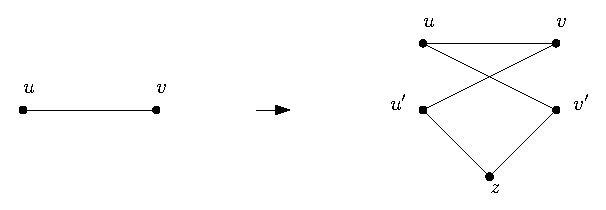
\includegraphics{img/triangle-free-colorful-construction.eps}
	\caption{Postup od $G_2$ na $G_3$}
	\label{triangle-free-colorful-construction}
\end{figure}

\subsection{Vybíravost}

\df (Barvení ze seznamů) Graf je obarvitelný ze seznamů $S_v$ povolených barev 
pro každý vrchol, pokud lze vybrat pro každý vrchol barvu z jeho seznamu 
takovou, že sousední vrcholy mají různou barvu.

\df (Vybíravost) Graf je $k$-vybíravý, pokud ho lze obarvit z libovolných
seznamů délky
$k$, značíme $\ch(G) = k$.

\poz Barevnost je speciální případ vybíravosti, speciálně když jsou všechny
seznamy stejné.

\vt (Thomassen) Každý rovinný graf je 5-vybíravý.

\dk Zavedeme indukční předpoklad: 

{\it Pro rovinný graf $G$, který se skládá z vnějšího cyklu $C$, na kterém jsou 
	dva sousední vrcholy předbarvené, a vnitřní stěny jsou triangulace, lze 
	rozšířit toto předbarvení na celý graf pokud všechny vrcholy na $C$ mají 
seznam délky alespoň $3$ a všechny vnitřní vrcholy alespoň $5$.}

Graf tedy doplníme na triangulaci, určíme vnější stěnu a hodíme graf do indukce 
podle počtu vrcholů. Pokud má graf chordu, rozdělíme ho podle ní na dvě 
poloviny, aplikujeme indukci na každou zvlášť, nejdříve však na půlku, která má 
předbarvené vrcholy. Pokud chordu nemá: předpokládáme $C=\{v_1, \dots, v_k\}$ 
vrcholy na vnější stěně, $v_1$ a $v_2$ jsou již obarvené, obarvíme $v_k$: 
zvolíme dvě barvy ze seznamu $v_k$, vyškrtáme
je z jeho sousedů uvnitř grafu $u_i$ (ti měli 5, zbydou jim alespoň 3, tak 
akorát do indukce) a graf pustíme dál do indukce bez $v_k$ (viz obrázek).  
Následně obarvíme $v_k$ barvou, kterou nepoužil $v_{k-1}$, takové máme dvě, 
které jsme si vyškrtali ze sousedů $u_i$ kromě $v_{k-1}$!

\noindent
\begin{figure}[h!]
	\centering
	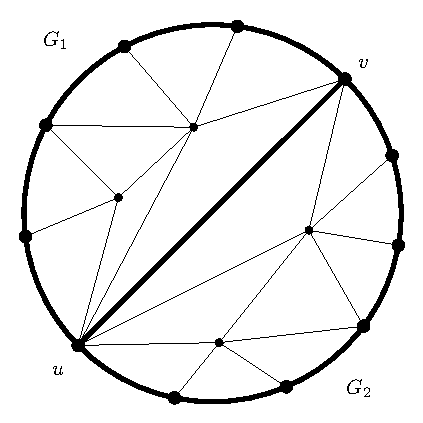
\includegraphics{img/thomassen-chord.eps}
	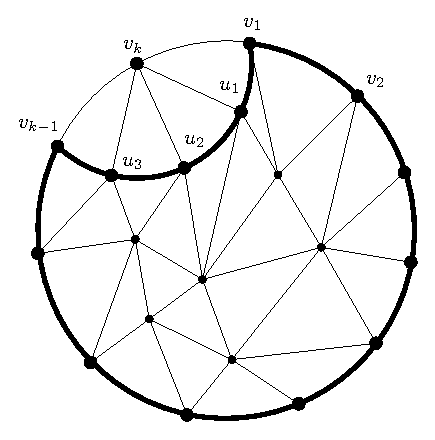
\includegraphics{img/thomassen-induction.eps}
	\caption{Postup indukce v grafu s chordou a bez ní.}
\end{figure}

\df Definujme hranovou barevnost a hranovou vybíravost grafu $G$ jako vrcholovou
barevnost a vybíravost jeho linegrafu, tedy $\L(G)$. Značíme $\chi'(G)$ a
$\ch'(G)$.

\vt (List Coloring Conjecture) Pro každý graf platí $\chi'(G) = ch'(G)$.

\vt (Galvin) Pro každý bipartitní graf platí $\chi'(G) = ch'(G)$.

\subsection{Kernel}

\df (Kernel) Nezávislá množina $U$ v orientovaném grafu je {\it kernel}, pokud 
každý vrchol $v\in G \setminus U$ má hranu $vu$ do nějakého vrcholu $u\in U$.  
{\it Alternativně: každý vrchol je v kernelu, nebo do něj má hranu.}

\lm Nechť $G$ je graf a $D$ jeho orientace a každý vrchol má méně výstupních 
hran, než barev ve svém seznamu, a každý indukovaný podgraf $D$ má kernel, potom
má $G$ seznamové obarvení.

\dk Pro barvu $\alpha$ vezmu graf indukovaný vrcholy, které mají $\alpha$ ve 
svých seznamech. Z předpokladů tento graf má kernel -- obarvím kernel barvou 
$\alpha$, odstraním a pokračuji indukcí (graf se zmenšil, některým vrcholům se 
zmenšily seznamy, ale také ekvivalentně odchozí stupně -- předpoklady stále 
platí).


\section{Regulární grafy}
\df {\it \emph{Regulární graf} je graf, jehož všechny vrcholy mají stejný stupeň. Graf je $k$\emph{-regulární}, je-li stupeň všech jeho vrcholů $k$.}

\begin{itemize*}
\item 0-regulární grafy se skládají z izolovaných vrcholů
\item 1-regulární grafy jsou disjunktním sjednocením hran
\item 2-regulární grafy jsou disjunktním sjednocením cyklů a nekonečných cest
\item 3-regulární grafy nazýváme kubické, patří mezi ně např. Petersen
\end{itemize*}

\vt (o vlastních číslech) {\it Graf $G$ je $k$-regulární $\Leftrightarrow$ matice sousednosti $G$ má vlastní číslo $k$ a odpovídající vlastní vektor $(1,\dots,1).$ 
$k$-regulární graf je souvislý $\Leftrightarrow$ vlastní číslo $k$ má násobnost 1.}

\subsection{Silně regulární grafy}
\df {\it \emph{Silně regulární graf} je $d$-regulární, $\forall$ hranu $xy\in E$ $\exists!e$ vrcholů $u: ux,uy\in E$ a $\forall$ nehranu $xy\not\in E$ $\exists!f$ vrcholů $u: ux,uy\in E$.}

Abychom mohli zanedbat triviální případy, dodáváme $f>0$ a $G\neq K_n$.
Příkladem silně regulárního grafu je úplný bipartitní graf se stejně velkými
partitami ($e=0$). Nejmenším nebipartitním silně regulárním grafem je
pěticyklus ($e=0$, $f=1$). Nejmenší graf, který je regulární, ale není silně
regulární je šesticyklus.

\vt (Friendship theorem) {\it Nechť $G=(V,E)$ je graf, že každé dva vrcholy $u,v$ mají právě jednoho společného souseda. Pak existuje $u$, že $\deg(u) = n-1$.}

Neboli Friendship theorem tvrdí, že takový silně regulární graf musí vypadat jako
mlýn (hromádka trojúhelníků, které se stýkají v jednom centrálním vrcholu).

\subsection{Moorovy grafy}

Moorovy grafy jsou $r$-regulární grafy bez krátkých cyklů (délky 3 a 4) s nejmenším možným počtem vrcholů. Obecně se definují i pro jiný girth (délku nejkratší kružnice), definice z LAKu je následující:

\df Moorův graf je takový $r$-regulární graf bez troj- a čtyř-úhelníků, kde $|V| = 1 + r + r(r-1) = r^2 + 1$.

Konstrukcí lze ukázat, že menší počet vrcholů už implikuje malý cyklus, nebo rozbije $r$-regulárnost.

\vt Moorův graf existuje pro $r=1,2,3,7$, pro $r=57$ se neví (otevřený problém) a pro žádné další $r$ neexistuje.

\dk (Idea) Mějme graf $G$ Moorův a $A$ jeho matici sousednosti. Zapišme druhou 
mocninu $A$ jako stupeň na diagonále a prohozené 0 a 1 jinde a upravme:
\begin{align}
	&A^2 = r\In + ({\bf J}_n- A - \In) \\
	\label{moorova-matice}&A^2 + A + (1-r)\In = {\bf J}_n
\end{align}
Dále pro nějaké $\lambda\in \Sp(A)$ a $x$ odpovídající vlastní vektor:
\begin{align}
	\label{moorova-mocnina}A^2 x = AAx = A\lambda x = \lambda A x = \lambda 
	\lambda x = \lambda^2 x
\end{align}
A dosadíme (\ref{moorova-matice}) za $A$:
\begin{align}
	{\bf J}_nx = (A^2 + A + (1-r)\In)x = (\lambda^2 + \lambda + (1-r))x
\end{align}
A tedy $(\lambda^2 + \lambda + 1 -r) \in \Sp(J)$. Vlastní čísla matice ${\bf J}_n$ 
(matice samých jedniček) ale známe, jsou to $\{0^{(n-1)}, n^{(1)}\}$. Zjevně pro 
$\lambda = r$ vyjde vlastní číslo $n$, je tedy potřeba vyřešit kvadratickou 
rovnici s parametrem $r$:
\begin{align}
	\lambda^2 + \lambda + 1 - r = 0
\end{align}
Jak na to půjdeme? Vyjádříme si $\lambda$ známým vzorečkem pro kořeny:\footnote{$D=b^2-4ac,\quad x_{1,2} = {-b \pm \sqrt D \over 2a}$}
\begin{align}
	\lambda_{1,2} = \frac{-1\pm \sqrt{1-4(1-r)}}{2} = \frac{-1\pm\sqrt{4r-3}}{2}
\end{align}
Násobnost označíme $m_1, m_2$. Stopa matice je suma vlastních čísel včetně
násobností, ale také součet čísel na diagonále. Protože matice sousednosti $A$
má na diagonále vždy nuly, platí rovnice:


\begin{align}
	\Tr(A) = r+m_1\lambda_1 + m_2\lambda_2 = 0
\end{align}
Nejdříve
upravíme do formy (násobení dvěma a přeskupení):
\begin{align}
	2r - \sqrt{4r-3}(m1-m2) - \underbrace{(m_1+m_2)}_{m_1+m_2=n-1=r^2} &= 0\\
	2r - r^2 + \sqrt{4r-3}(m_1 - m_2) &= 0 
	\label{4-2:rovnice}
\end{align}
Moorův graf je $r$-regulární, $r\in\N$, tedy máme dvě možnosti:
\begin{enumerate}
	\item $\sqrt{4r-3} \not\in \Q$: potom $m_1 = m_2$ a tedy $r = 2$.
	\item $\sqrt{4r-3} = s \in \Q$, což implikuje\footnote{Odmocnina z celého čísla je
  vždy celé číslo či iracionální číslo, nikdy zlomek.} $s \in \N$.
  Substitucí $4r - 3 = s^2$ do rovnice \ref{4-2:rovnice} získáme
	$s \in \set{1, 3, 5, 15}$, což dává $r \in \set{1, 3, 7, 57}$.
\end{enumerate}
\qed


\subsection{Regularita a Hamiltonovskost}
\vt (Dirac) {\it Máme-li souvislý graf $G$, $n \ge 3$ a stupeň každého vrcholu je alespoň $n\over 2$, pak je $G$ hamiltonovský.} 

Důkaz vezme nejdelší cestu v $G$ a hledá se spor s tím, že je nejdelší. Diracovu větu použijeme v důkazu následující věty od Nash-Williamse. 

\vt (Nash-Williams) {\it Každý $k$-regulární graf na $2k+1$ vrcholech obsahuje Hamiltonovskou kružnici.}

\dk Mějme $k$-regulární graf $G$ na $2k+1$ vrcholech. Přidáme k němu nový vrchol $w$ a spojíme ho se všemi vrcholy $G$. Výsledný graf $H$ má $2k+2$ vrcholů s minimálním stupněm $k+1$. Dle Diracovy věty je $H$ Hamiltonovský. Odebráním $w$ z $H$ získáme v $G$ Hamiltonovskou cestu $v_0v_1\dots v_{2k}$.

\begin{wrapfigure}{R}{6cm}
\centering
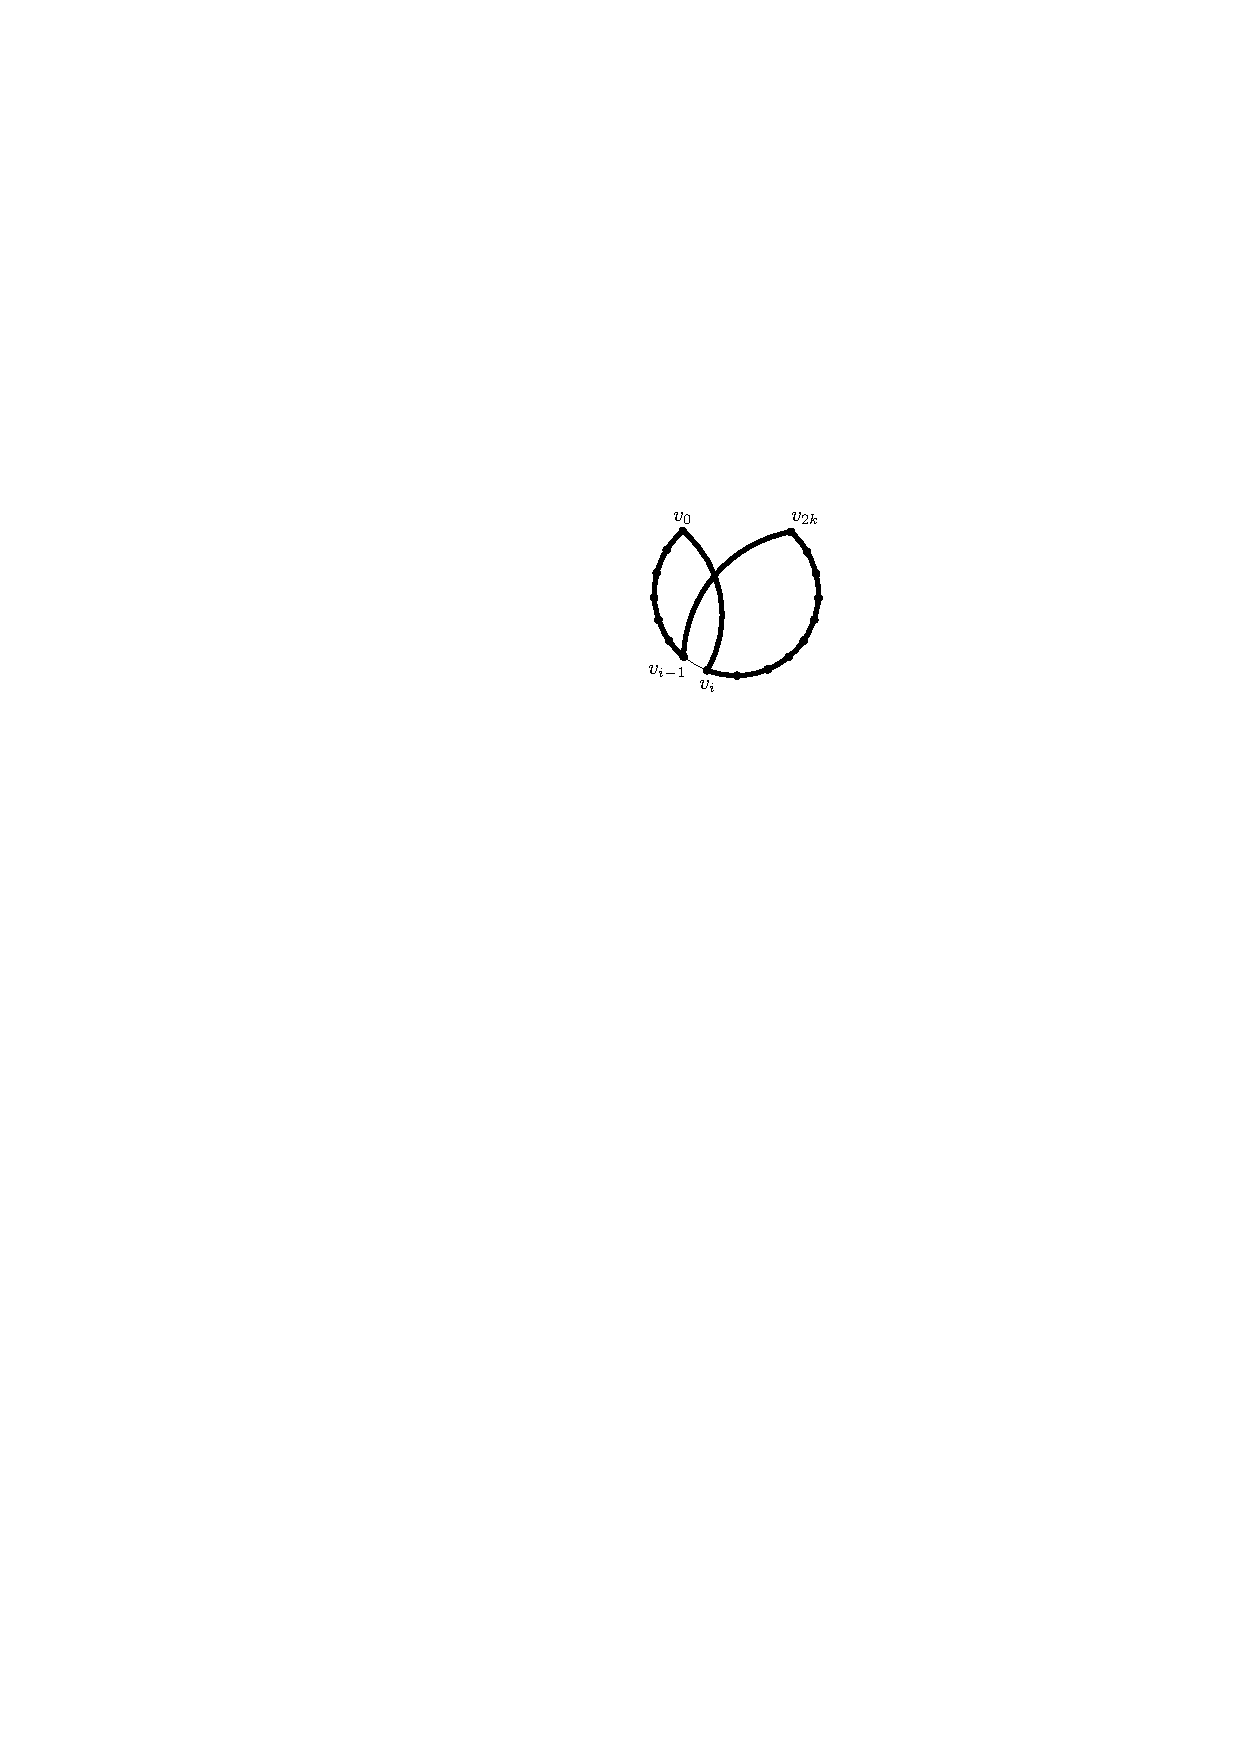
\includegraphics[width=5cm]{img/nash-williams4.pdf}
\caption{Triviální případ}
\label{dk:nw-triv}
\end{wrapfigure}

Předpokládejme že neexistuje dvojice na sousedních vrcholů $v_{i-1}v_i$, přes které by šla uzavřít kružnice (viz Obrázek \ref{dk:nw-triv}). Pak ale nutně platí, že když $v_0v_i \in E$, pak $v_{i-1}v_{2k} \not\in E$. Vrchol $v_{2k}$ má $k$ sousedů, ale nesmí mezi nimi být žádné vrcholy, jejihž pravý soused je spojen s $v_0$. Jinými slovy, $v_0$ nám vyblokuje $k$ vrcholů, do kterých nesmí vést hrana z $v_{2k}$ a ten sousedí se všemi ostatními. Tedy, když $v_0v_i \not\in E$, pak $v_{i-1}v_{2k} \in E$ (tuto vlastnost použijeme později).

\textbf{Případ (i)} $v_0$ sousedí právě s vrcholy v první polovině cesty a $v_{2k}$ právě s vrcholy v druhé polovině cesty. Pak musí existovat dvojice vrcholů $v_i,v_j$ v první polovině cesty, mezi kterými nevede hrana. Kdyby vedla hrana mezi každými dvěma vrcholy v první polovině cesty, pak by byl stupeň $v_k$ vyšší, než $k$. Protože stupeň $v_i$ je $k$, existuje $v_l$ v druhé polovině cesty tž. $v_iv_l \in E$. Pak najdu HK (viz Obrázek \ref{dk:nw-i}).

\textbf{Případ (ii)} Existuje vrchol $v_i$ takový, že $v_{i+1}v_0 \in E$, $v_iv_0 \not\in E$. Pak podle vlastnosti dokázané výše je $v_{i-1}v_{2k} \in E$. Potom $G$ obsahuje $2k$-cyklus $v_{i-1}v_{i-2}\dots v_0v_{i+1}\dots v_{2k}$ (viz Obrázek \ref{dk:nw-ii}). Přejmenujme $2k$-cyklus $C$ na $u_1u_2\dots u_{2k}$ a $u_0$ bude vrchol $G$, který v $C$ není. Potom $u_0$ nemůže sousedit se dvěma sousedními vrcholy $C$ (jinak by existovala HK) a tedy sousedí s každým druhým vrcholem $C$, řekněme s $u_1, u_3, \dots, u_{2k-1}$. Nahrazením $u_{2j}$ za $u_0$ ($\forall j$) dostaneme jiný maximální cyklus v $G$ a tedy $u_{2j}$ musí mít sousedy $u_1, u_3, \dots, u_{2k-1}$ (stejný argument jako v předchozí větě). Pak ale $u_1$ musí sousedit s $u_0, u_2, \dots, u_{2k}$ a tedy $\deg u_1 \ge k+1$, což je spor s $k$-regularitou. Tudíž je $G$ Hamiltonovský.
\qed

\begin{figure}[h]
\centering
\begin{subfigure}{7.5cm}
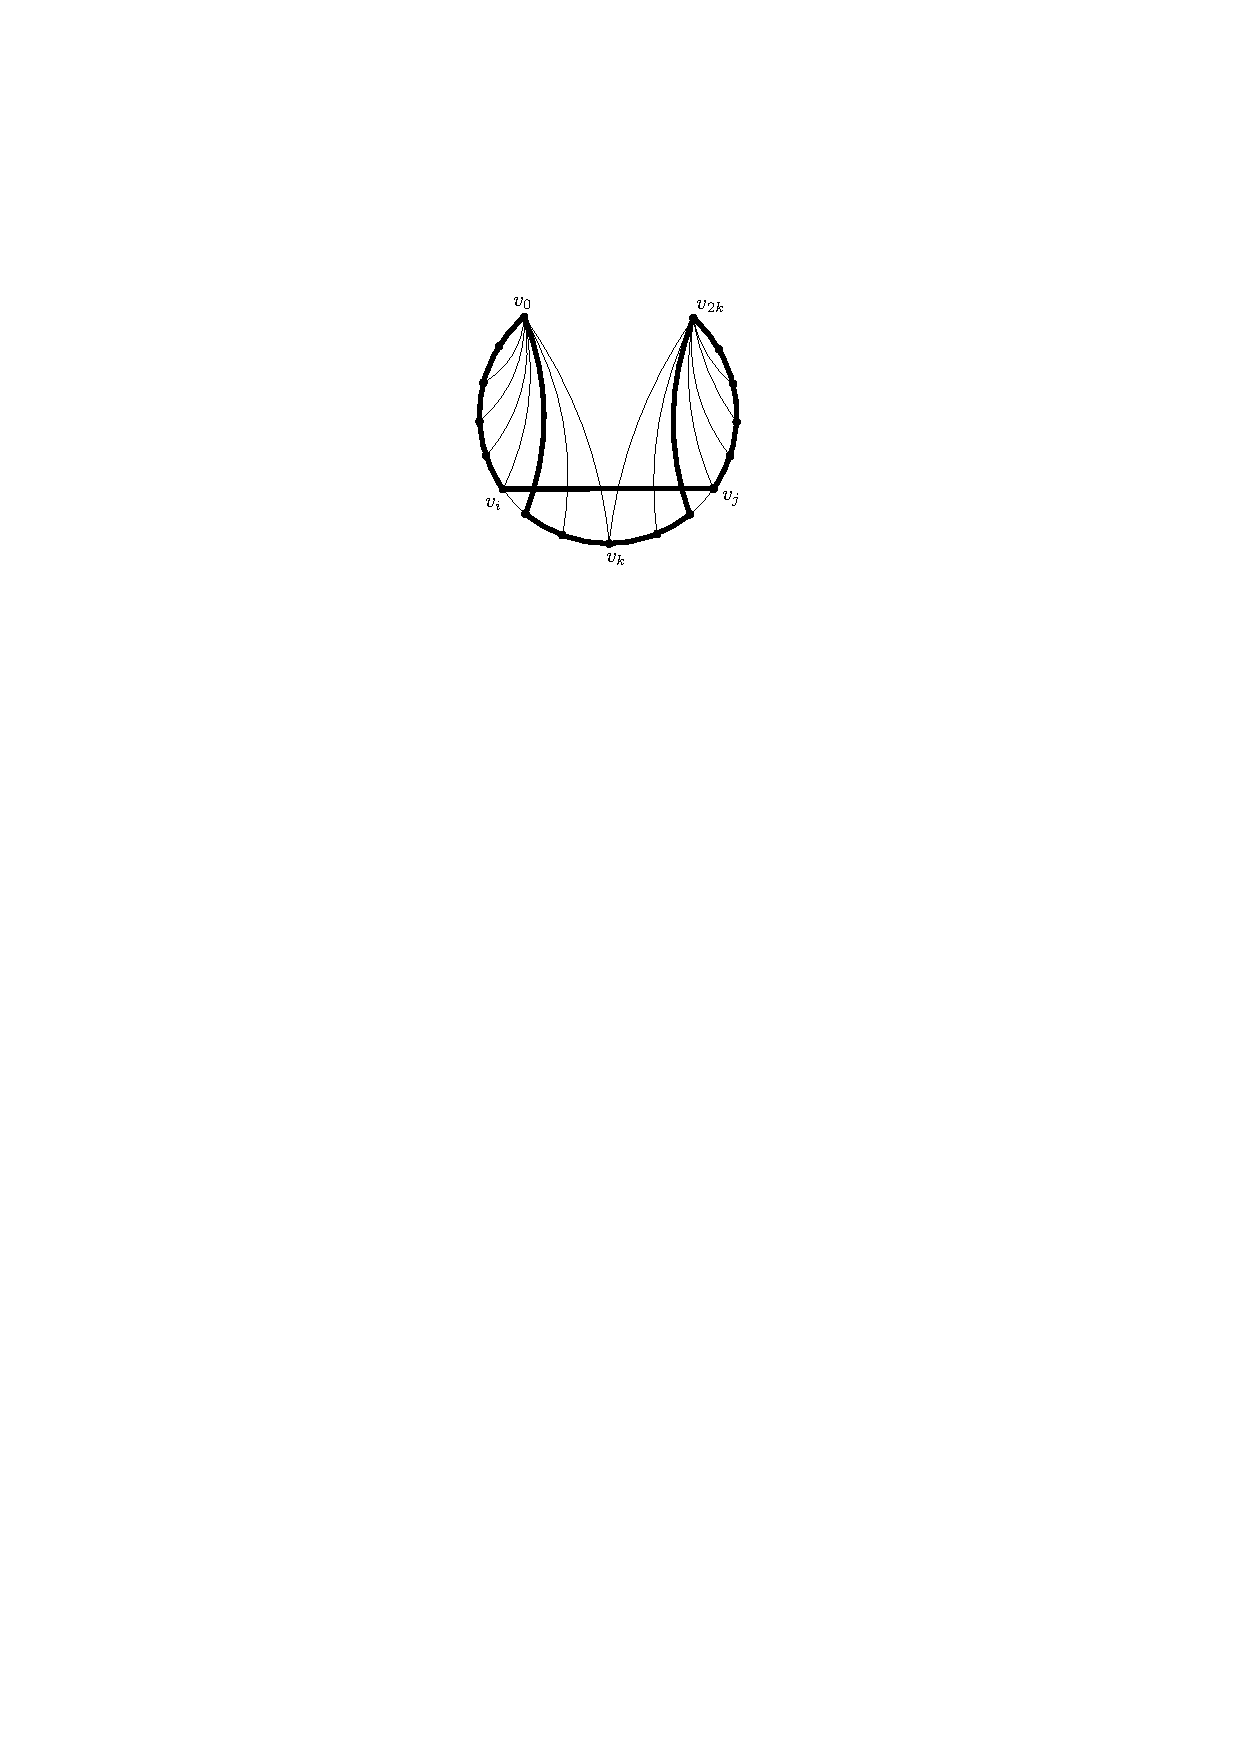
\includegraphics[width=7.5cm]{img/nash-williams2.pdf}
\caption{Případ (i)}
\label{dk:nw-i}
\end{subfigure}
\hfill
\begin{subfigure}{7.4cm}
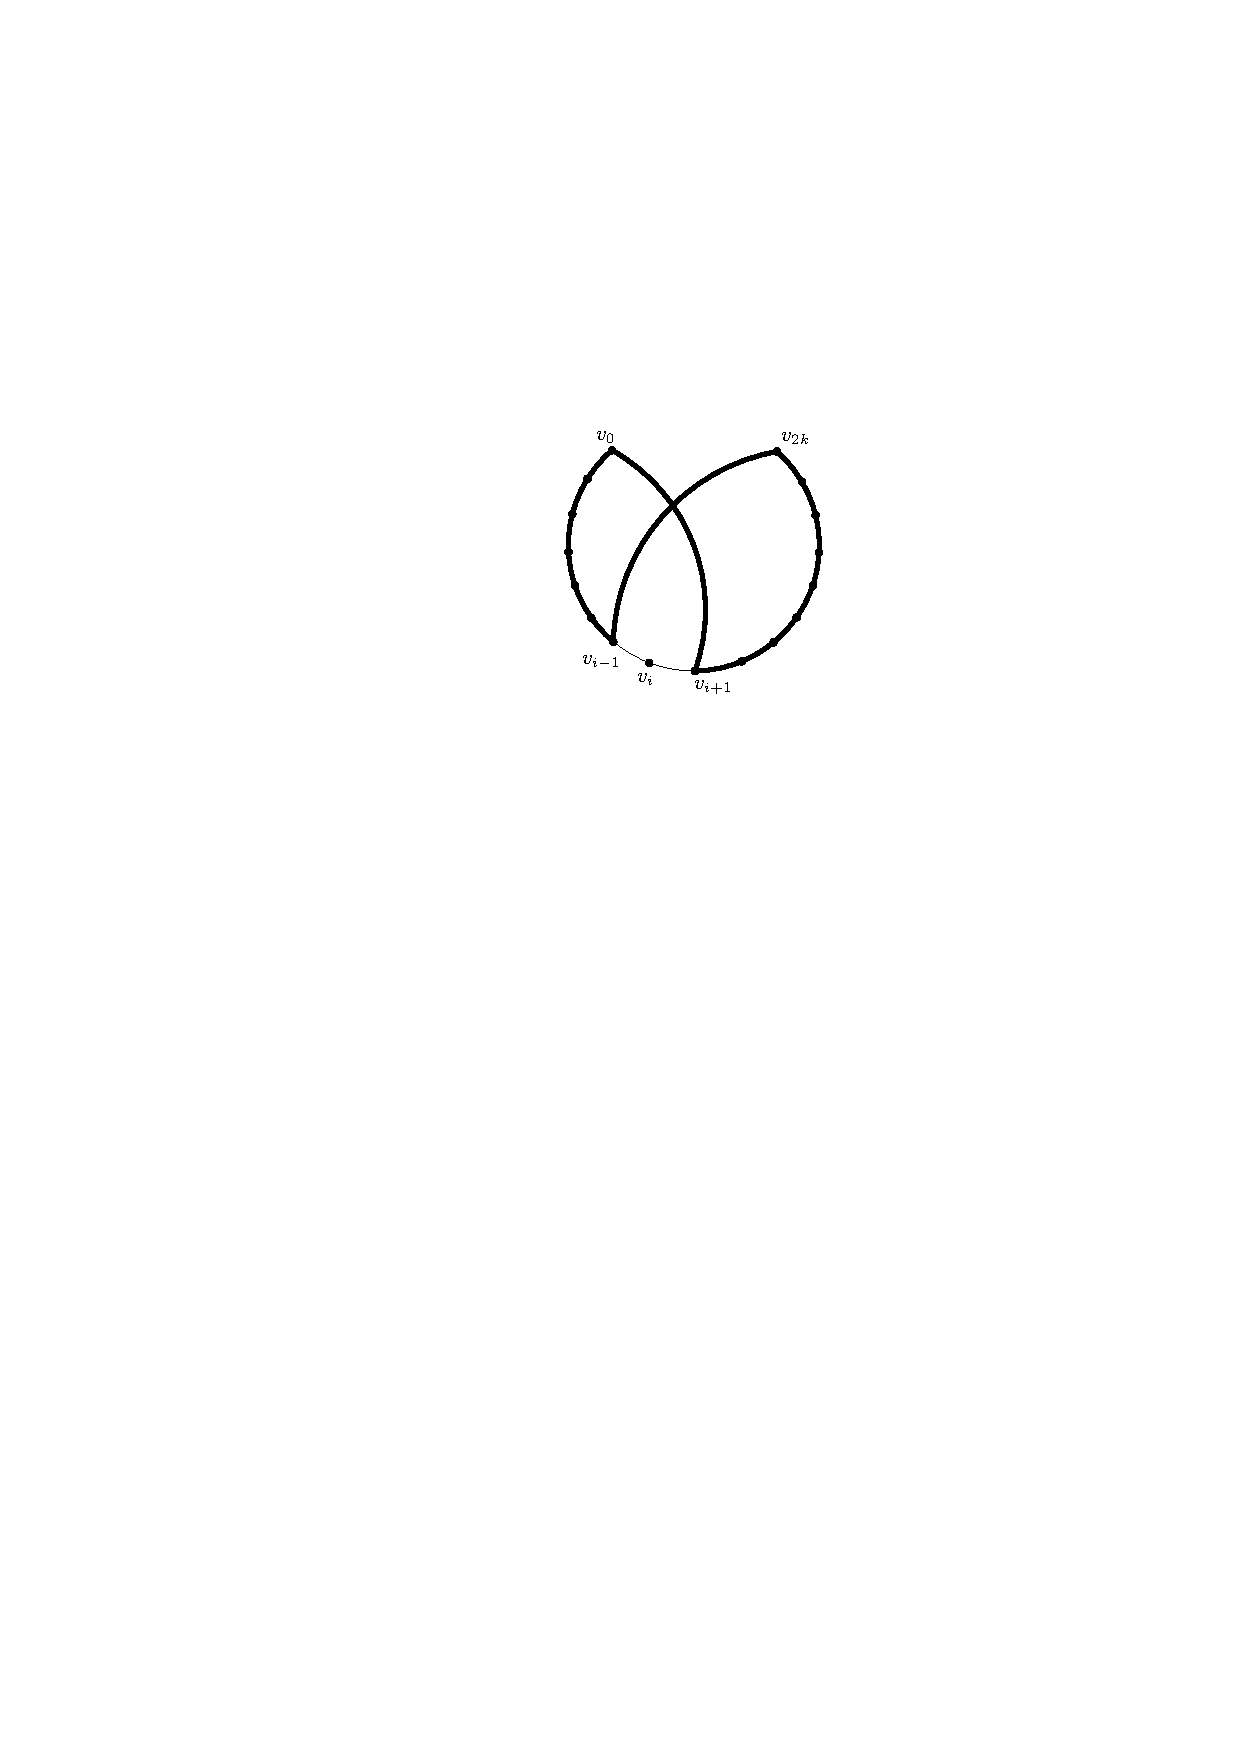
\includegraphics[width=7.5cm]{img/nash-williams3.pdf}
\caption{Případ (ii)}
\label{dk:nw-ii}
\end{subfigure}
\caption{Netriviální případy}
\end{figure}



\section{Souvislost grafů}
\section{Speciální vlastnosti orientovaných grafů}
\section{Speciální vlastnosti orientovaných grafů}

\label{silna-souvislost}

V orientovaných grafech se množiny hran skládají z uspořádaných dvojic vrcholů.
Oproti neorientovaným grafům rozlišujeme dva druhy souvislosti. Graf je slabě
souvislý, pokud je souvislá jeho symetrizace. Graf $G$ je silně souvislý, pokud
$\forall u,v \in V(G), u\neq v$ existuje orientovaná cesta z $u$ do $v$.
Analogicky definujeme silně souvislé komponenty (SSK) grafu $G$.

\subsection{Algoritmus pro hledání SSK}

Než popíšeme algoritmus, všimneme si nejprve několika vlastností orientovaných
grafů. Graf SSK je orientovaný acyklický graf. Proto v něm musí existovat
alespoň jedna zdrojová komponenta (do níž nevedou žádné hrany) a alespoň jedna
stoková komponenta (z níž nevedou žádné hrany). Kdybychom měli vrchol ze stokové
komponenty, mohli bychom z něj pustit DFS, který najde právě všechny vrcholy v
této SSK. Po odebrání této komponenty z grafu bychom našli novou stokovou
komponentu a pokračovali, dokud by nebyl celý graf rozdělen.

Nevíme sice, jak najít vrchol ze stokové komponenty, ale je jednoduché najít vrchol ze zdrojové komponenty -- stačí na $G$ spustit DFS (opakovaně, pokud neprošel všechny vrcholy). Vrchol, který opustíme jako poslední\footnote{Při zavedení DFS si obvykle zadefinujeme pořadí podle opouštění vrcholu, značíme $out(v)$.}, je určitě ve zdrojové komponentě. Je zjevné, že když otočíme orientaci všech hran v $G$, SSK se nezmění, pouze se ze stokových stanou zdrojové a naopak.

\lm {\it V grafu SSK $G$ vede hrana z komponenty $C_1$ do $C_2$, pak
$\max_{x\in C_1} out(x) > \max_{y\in C_2} out(y)$}

Z výše uvedeného již vyplývá jakým způsobem algoritmus pracuje: Nejprve obrátí orientaci všech hran v $G$ a najde pořadí $out(v)$ pro všechny vrcholy $G$. Poté opakovaně spouští DFS z ještě neprozkoumaných vrcholů, v pořadí od nejvyššího nalezeného $out(v)$.\footnote{Zápis algoritmu v pseudokódu je přejat z \url{http://mj.ucw.cz/vyuka/ads/25-grafy.pdf}.}

\begin{enumerate*}
\item Sestrojíme graf $G^T$ s obrácenými hranami
\item $Z \leftarrow$ prázdný zásobník
\item Pro všechny vrcholy $v$ nastavíme $komp(v) = 0$
\item Spouštíme DFS v $G^T$ opakovaně, než prozkoumáme všechny vrcholy. Kdykoliv přitom opouštíme vrchol, vložíme ho do $Z$. Vrcholy v zásobníku jsou tedy setříděné podle $out(v)$.
\item Postupně odebíráme vrcholy ze zásobníku $Z$ a pro každý vrchol $v$:
\item $\qquad$Pokud $komp(v) = 0$
\leftmargin=6cm
\indent
\item $\qquad\qquad$ Spustíme DFS($v$) v $G$, přičemž vstupujeme pouze do vrcholů s $komp(x) = 0$ a tuto hodnotu přepisujeme na $v$.
\end{enumerate*}

\dk Důkaz korektnosti algoritmu je zjevný z lemmatu a pozorování, která mu předchází. Algoritmus pouze spouští DFS a žádný vrchol neprojde vícekrát, takže se určitě zastaví. Časová i prostorová složitost jsou $\Theta(n+m)$.
\qed

Existuje i tzv. Tarjanův algoritmus pro hledání SSK, který je složitější a jeho časová i prostorová složitost je asymptoticky stejná (musí být, protože také volá DFS). Nemusí ovšem konstruovat graf s obrácenými hranami.

\subsection{Turnaje a hamiltonovské cesty}

\df (Turnaj) Turnaj je orientace úplného grafu.

\vt (O počtu Hamiltonovských cest) Existuje turnaj na $n$ vrcholech, který
obsahuje alespoň $n!/2^{n-1}$ hamiltonovských cest.

\dk Zorientujme graf nezávisle uniformě náhodně. Nechť máme permutaci $\pi$.
Jaká je pravděpodobnost, že daná permutace (tedy pořadí vrcholů) tvoří
orientovanou cestu? Máme $n-1$ hran na cestě, všechny mají permutací
předepsanou orientaci. Tedy $P(X_\pi)= 1/2^{n-1}$. Nechť $I_\pi$ je indikátor
tohoto jevu, pak $\E[I_\pi] = P(X_\pi) = 1/2^{n-1}$.

Spočítáme-li střední hodnotu počtu hamiltonovských cest, tedy součet indikátorů
přes všechny permutace, máme $n!/2^{n-1}$. Z vlastností střední hodnoty víme,
že existuje alespoň jeden graf, který má právě tolik (nebo více) hamiltonovských
cest.

\section{Algebraické vlastnosti grafů}

\subsection{Vlastní čísla grafu}

\df Vlastní čísla grafu jsou vlastní čísla matice sousednosti grafu. Množina 
vlastních čísel je {\it spektrum}, $\Sp = \{\lambda_1, \lambda_2, \dots\}$ a 
většinou se udává setříděná podle velikosti (tj. $\lambda_1$ je typicky 
největší vlastní číslo). Pro vlastní čísla platí $Ax = \lambda x$ a lze je 
vypočítat jako $\det(A - \lambda E) = 0$.

\subsection{Expandéry}

\vt (O vlastních číslech bipartitního grafu) Graf $G$ je bipartitní právě 
tehdy, když je jeho spektrum symetrické (vzhledem k nule). Pokud je navíc $G$ 
souvislý, stačí pouze $\lambda_{min} = -\lambda_{max}$.

\df Rodina expandérů $G_i$ je třída d-regulárních grafů rostoucích velikostí, 
kde každý graf má \uv{dobrou expanzí} (podle nějakého parametru).

\df (Expanze) \begin{itemize}
	\item Vrcholová expanze: $h_v(G) = \min_{S\subseteq V, |S|\leq n/2} 
	{|N(S)\setminus S| \over |S|}$.
	\item Hranová expanze: $h(G) = \min_{S\subseteq V, |S|\leq n/2} {|\delta S| 
	\over |S|}$, kde $\delta S$ značí hrany, které mají právě jeden vrchol v 
	$S$.
\end{itemize}

\poz (O hranové a vrcholové expanzi) $h_v(G) \leq h(G) \leq d \cdot h_v(G)$.

\vt (O vlastních číslech a expanzi) Pro $G$ $d$-regulární graf platí: $1/2(d - 
\lambda_2) \leq h(G) \leq \sqrt{d \cdot (d - \lambda_2)}$

\subsection{Konstrukce expandérů}

Ačkoliv například úplný graf je dobrý expandér ve smyslu, že má vysokou 
expanzi, bohužel s expanzí a velikostí roste neúnosně stupeň. Následující 
konstrukce vytváří grafy, které mají vyokou expanzi, ale konstantně malý 
stupeň.

\vt (Randomizovaná) Mějme $2n$ vrcholů. Pro $d$-regulární expandér zvolíme $d$ 
uniformě náhodných prefektních párování nad těmito vrcholy. Sjednocení těchto 
párování dává $d$-regulární graf, který je navíc dobrý expandér.

\vt (Prvočíselná) Nechť $p$ je prvočíslo a $V:=Z_p$. Definujeme $G_p=(V,E)$ s 
hranami $(x, x+1)$ a $(x,x^{-1})$ ($0^{-1}$). Pak $G_p$ je rodina dobrých 
expandérů.

\vt (Margulis) Nechť $G_m=(V,E)$ a $V=\Z_m \times \Z_M$. Definujeme hrany pro 
$4$-regulární graf jako: $(x\pm y, y)$ a $(x,y\pm x)$. Pak $G_m$ je rodina 
dobrých expandérů.

\df (Zig-Zag) Nechť $G$ je $g$-regulární graf a $H$ je $h$-regulární graf na $d$ 
vrcholech. Definujeme $G \zz H$ následujícím způsobem:
\begin{enumerate}
	\item Říkejme, že hrany z $G$ jsou {\bf\color{red}červené} a hrany z $H$ 
		jsou {\bf\color{blue}modré}.
	\item Vrcholy $G$ nahradíme grafy $H$ tak, že každému vrcholu $H$ přiřadíme 
	jednu hranu $G$. Protože $G$ je $g$-regulární a $H$ má právě $g$ vrcholů, 
	nyní každý vrchol má právě jednu hranu z $G$.
	\item Pro každou cestu tvaru 
		{\bf\color{blue}modrá}-{\bf\color{red}červená}-{\bf\color{blue}modrá} 
		vytvoříme {\bf\color{magenta}růžovou} hranu z prvního vrcholu do 
		posledního vrcholu.
	\item Odstraníme z grafu {\bf\color{blue}modré}-{\bf\color{red}červené} 
		hrany.
\end{enumerate}
Ukázka konstrukce je na obrázku \ref{zigzag-konstrukce}. Pro názornost není graf
$H$ regulární (nepodařilo se mi najít lepší příklad). Příklad je převzat z webu
\footnote{
\url{http://math.stackexchange.com/questions/454162/clearing-doubt-over-a-definition}}.

\begin{figure}
\centering
\begin{subfigure}{7.5cm}{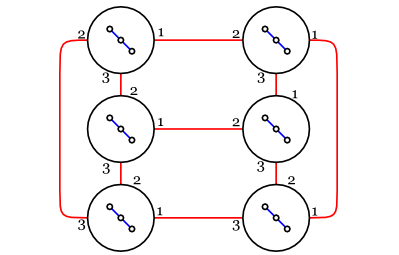
\includegraphics[width=\textwidth]{img/zigzag1.png}}\caption{Vložení 
$H$ do $G$}\end{subfigure}
\begin{subfigure}{7.5cm}{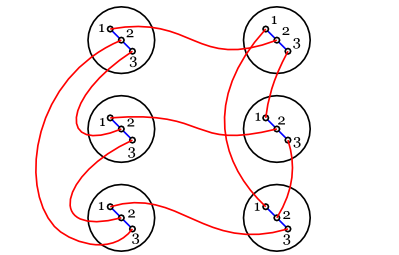
\includegraphics[width=\textwidth]{img/zigzag2.png}}\caption{Napojení 
hran $G$ na vrcholy $H$}\end{subfigure}
\begin{subfigure}{7.5cm}{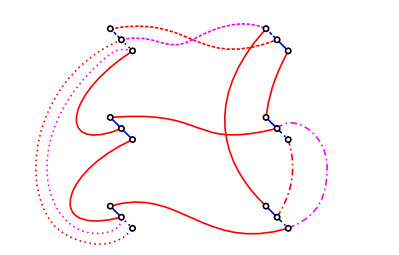
\includegraphics[width=\textwidth]{img/zigzag3.png}}\caption{Tvorba 
růžových hran}\end{subfigure}
\begin{subfigure}{7.5cm}{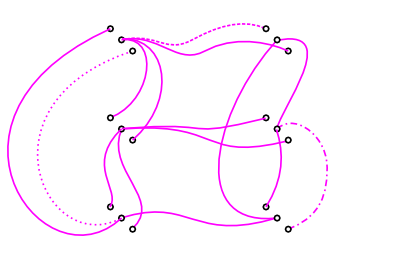
\includegraphics[width=\textwidth]{img/zigzag4.png}}\caption{Výsledek}\end{subfigure}
\caption{Příklad Zig-Zag součinu. Pro jednoduchost není $H$ regulární, na funkci
to ale nic nemění.}
\label{zigzag-konstrukce}
\end{figure}

\poz Díky této konstrukci máme graf, který zachovává velikost $G$ (dokonce ji 
zvětšuje), ale dědí stupeň po grafu $H$ (pokud stupeň byl $h$, nyní bude $h^2$ 
-- to sice není úplně dobré, ale mohlo by to být horší).

\vt (Zig-Zag) Nechť $H$ je dobrý $d$-regulární expandér, $G_1 := H^2$. Potom 
rodina grafů $G_{i+1} := G_i\zz H$ je dobrý expandér.

\section{Teorie párování}

\section{Ramseyova teorie}
Ramseyova teorie zkoumá především výskyt zajímavých struktur na velmi velkých grafech. Ramseyových vět existuje hned několik, začneme ovšem jinou extremální větou a to Turánovou. Hlavními výsledky v Ramseyově teorii jsou Hales-Jewett a Van der Waerdenova věta.

\subsection{Turánova věta}

\df Turánův graf $T(n,r)$ {\it je graf na $n$ vrcholech, které byly rozděleny do $r$ skupin, jejichž velikost se liší nejvýš o 1. Hrana vede mezi každými dvěma vrcholy, které nejsou ve stejné skupině.}

Turánovy grafy jsou pokus o konstrukci hranově extremálních grafů neobsahujících podgraf $K_{r+1}$. Turánova věta nám pak říká, že turánovy grafy mají skutečně maximální možný počet hran.

\vt (Turánova, verze 1) {\it Ze všech grafů na $n$ vrcholech, které neobsahují $K_{r+1}$ jako podgraf má $T(n,r)$ nejvyšší počet hran.}

\vt (Turánova, verze 2) {\it Nechť $G$ je graf na $n$ vrcholech neobsahující $K_{r+1}$ jako podgraf. Pak počet hran $G$ je nejvýš ${r-1\over r}\cdot{n^2\over 2} = \left(1-{1\over r}\right)\cdot{n^2\over 2}$.}

\dk (Turánovy věty): Předpokládejme, že $G$ je graf neobsahující $K_{r+1}$ s
maximálním počtem hran. V první části důkazu ukážeme, že $G$ musí být úplný
$r$-partitní graf, v druhé části že se velikost jednotlivých partit může lišit
nejvýš o 1.

\textbf{Část 1.} Graf $G$ neobsahuje trojici vrcholů $u$, $v$, $w$ tž. hrana
vede pouze mezi $u$ a $v$. To dokážeme tak, že buď smažeme $w$ a zkopírujeme
$u$, nebo smažeme $u$ a $v$ a zkopírujeme dvakrát $w$, čímž dostaneme graf s
více hranami. Z toho plyne, že můžeme vrcholy $G$ rozdělit do tříd ekvivalence
na základě nesousednosti (dva vrcholy jsou ve stejné třídě, když mezi nimi
nevede hrana). Třídy ekvivalence tvoří partity a $G$ je tedy úplný
multipartitní graf. Čím více partit, tím více hran, takže $G$ je úplný
$r$-partitní graf.

\begin{figure}[h]
\centering
\begin{subfigure}{8cm}
\begin{subfigure}{3cm}
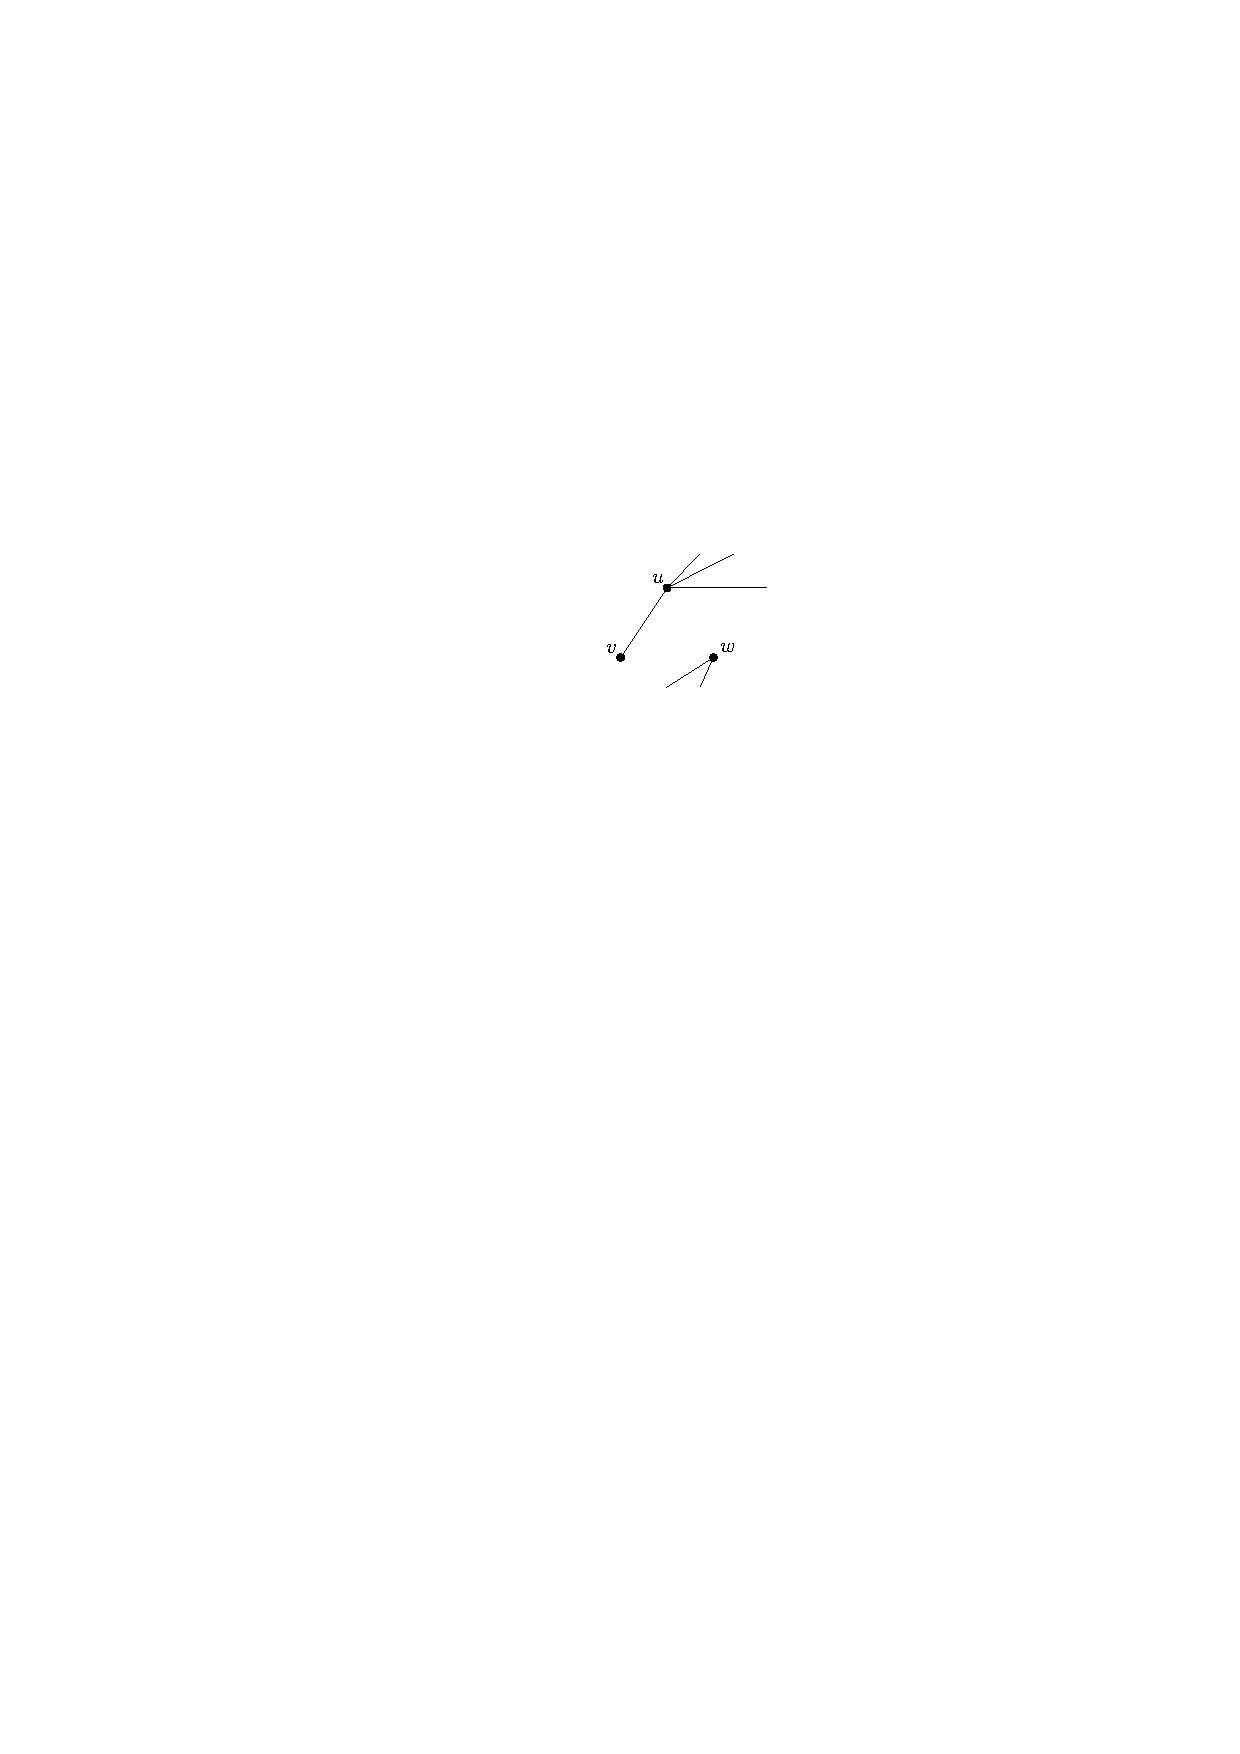
\includegraphics[width=3cm]{img/turan1.pdf}
\end{subfigure}
\hspace{0.5cm}$\Rightarrow$\hspace{0.5cm}
\begin{subfigure}{3cm}
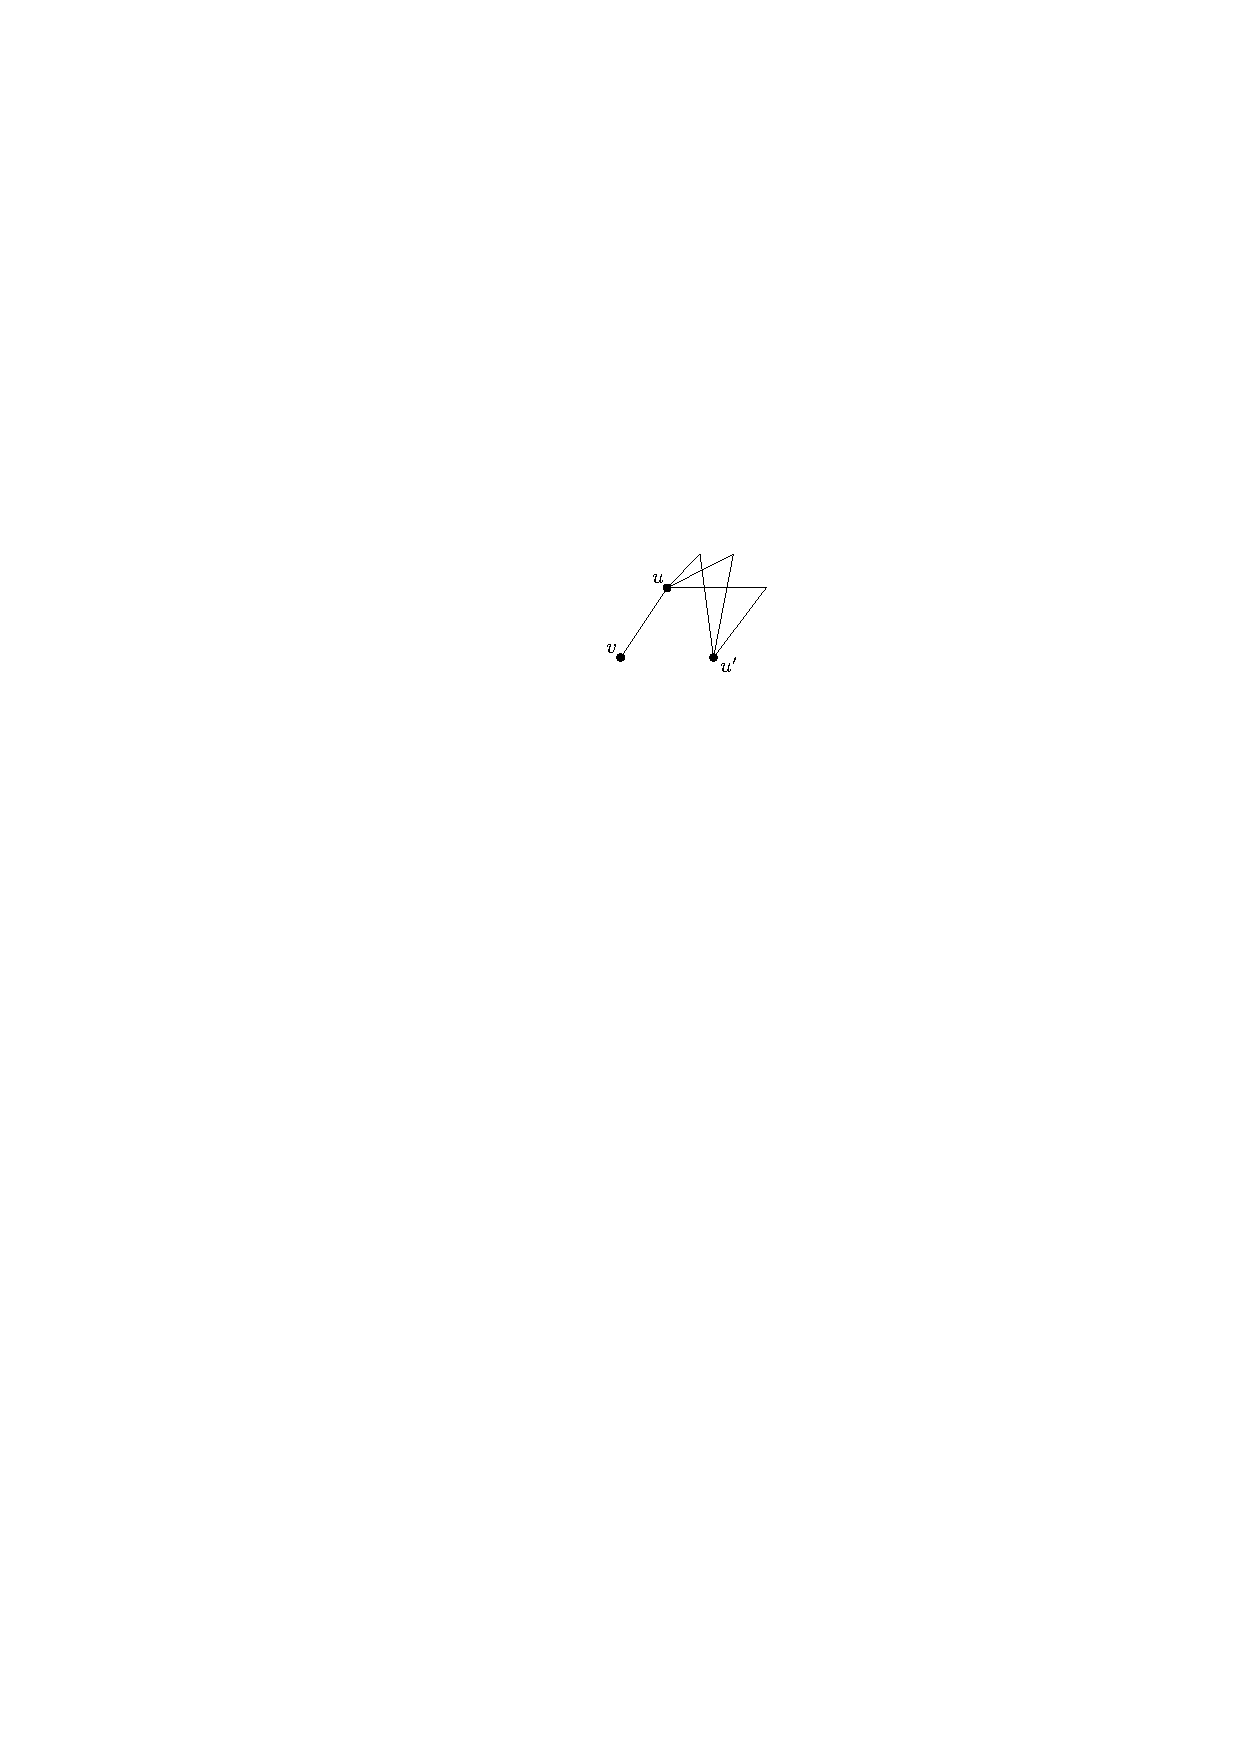
\includegraphics[width=3cm]{img/turan2.pdf}
\end{subfigure}
\caption{$d(w) < d(u)$}
\end{subfigure}
\hfill
\begin{subfigure}{8cm}
\begin{subfigure}{3cm}
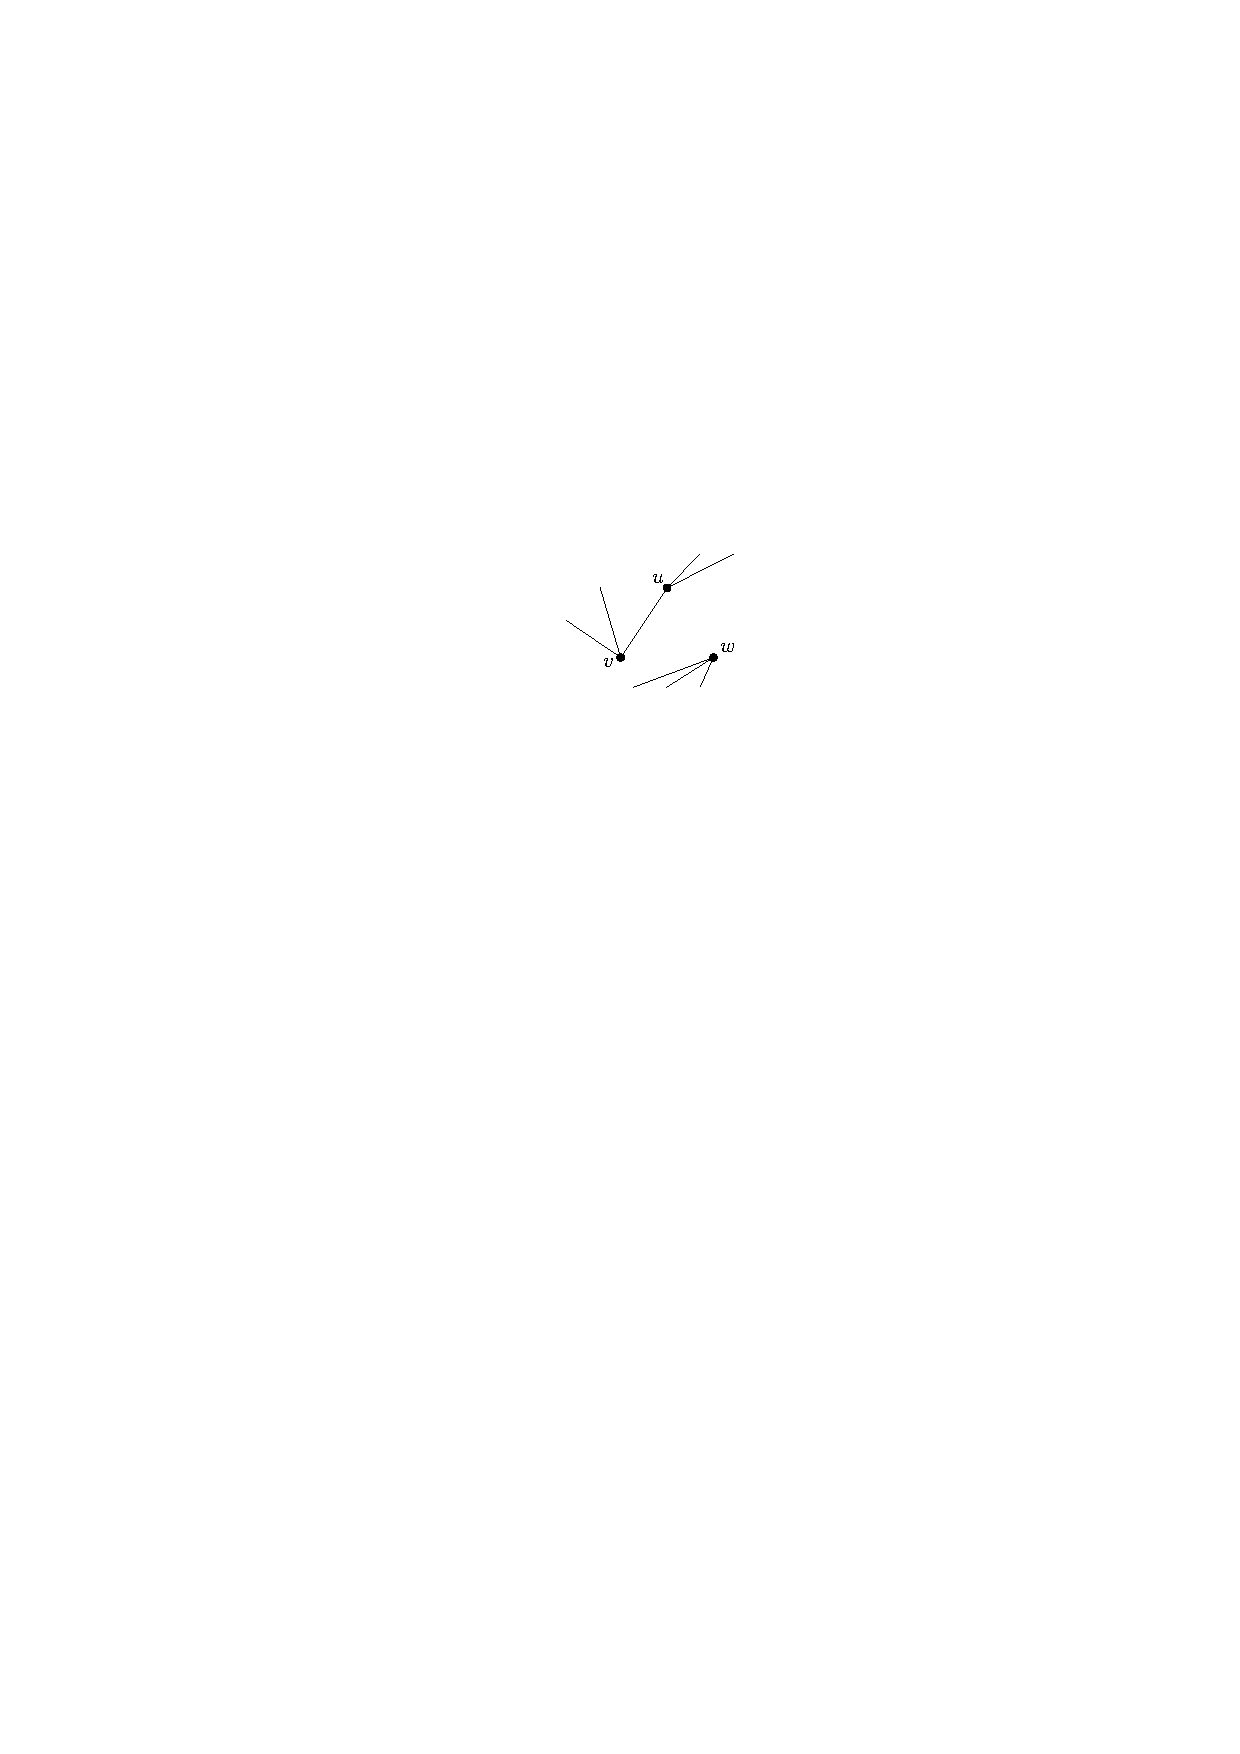
\includegraphics[width=3cm]{img/turan3.pdf}
\end{subfigure}
\hspace{0.5cm}$\Rightarrow$\hspace{0.5cm}
\begin{subfigure}{3cm}
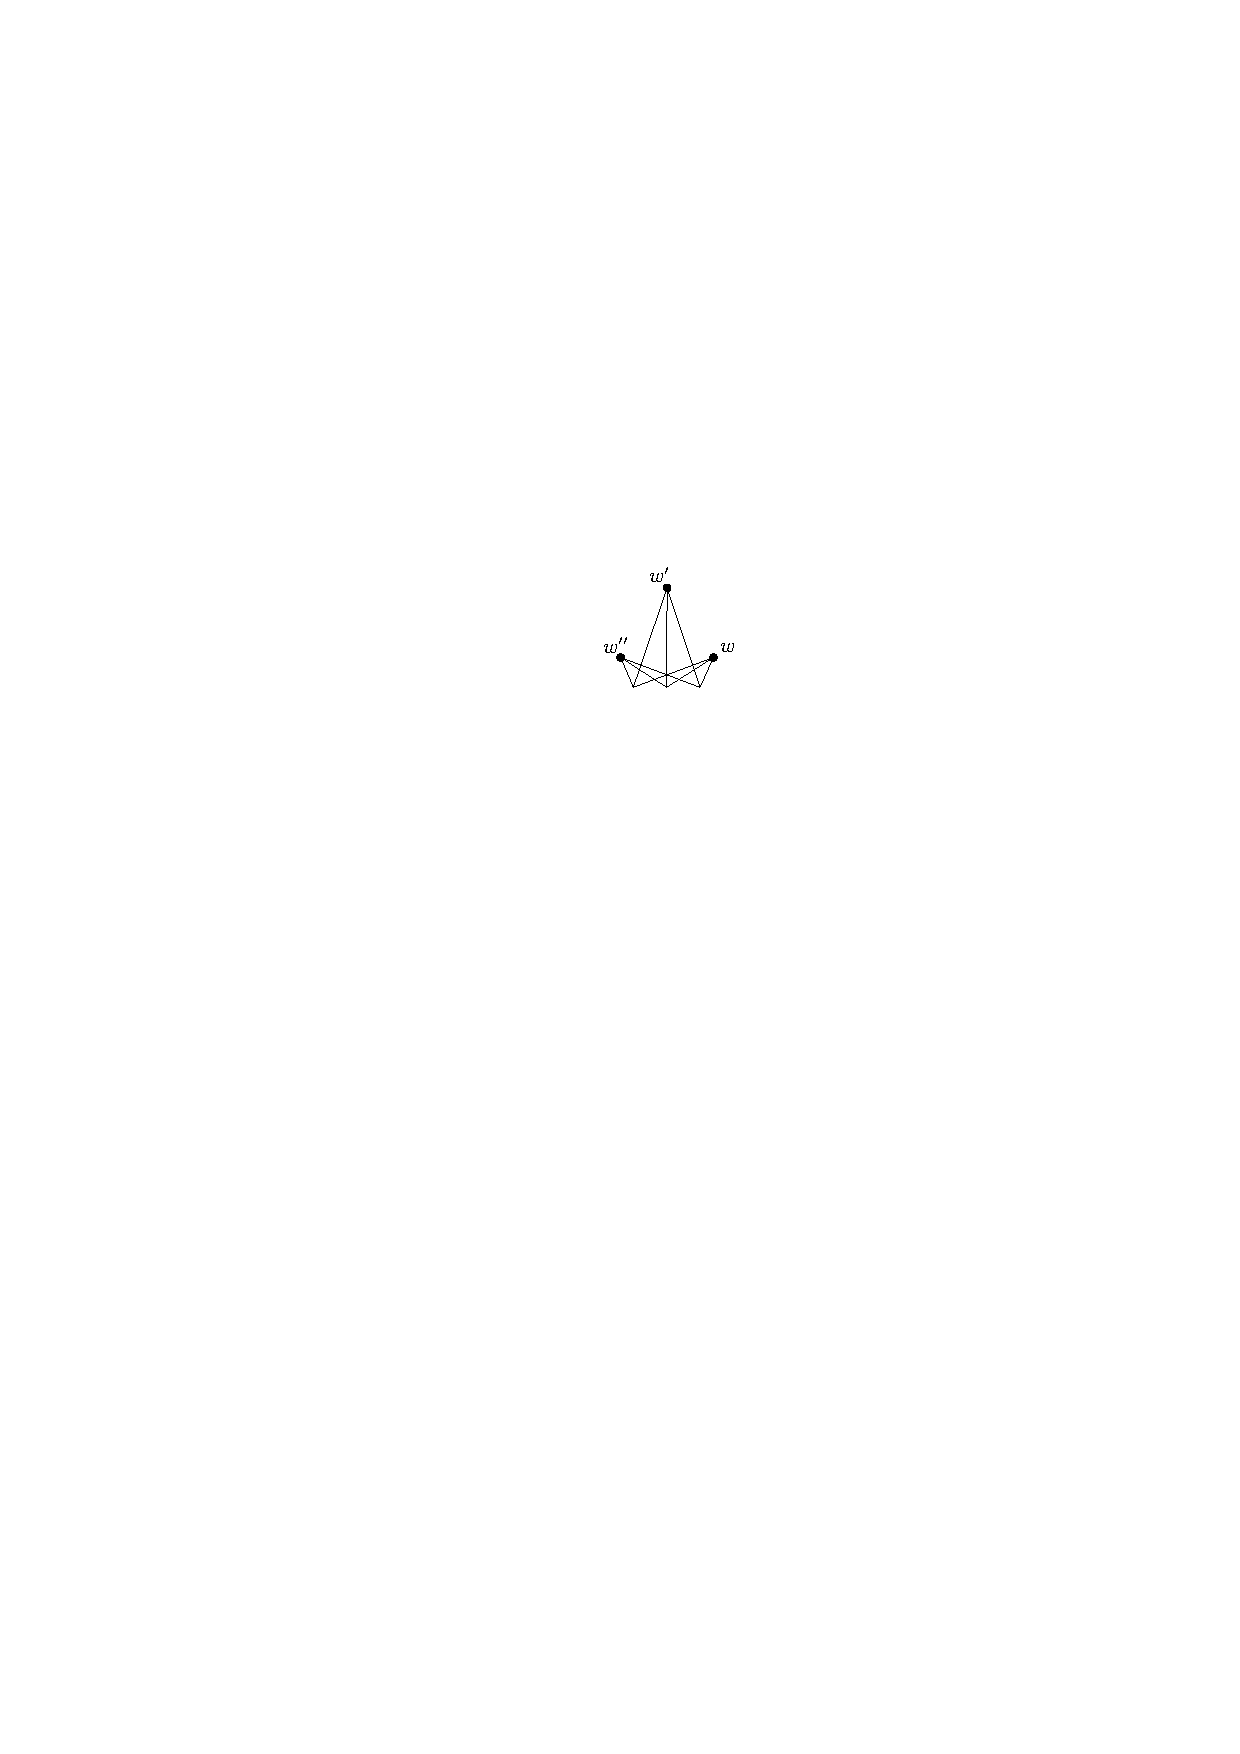
\includegraphics[width=3cm]{img/turan4.pdf}
\end{subfigure}
\caption{$d(w) \ge d(u)$ a $d(w) \ge d(v)$}
\end{subfigure}
\caption{Důkaz Turánovy věty, část 1.}
\end{figure}

\textbf{Část 2.} Mějme partity $A$ a $B$ tž. $|A| > |B| + 1$. Pak přesunem
vrcholu z $A$ do $B$ ztratíme $|B|$ hran, ale získáme $|A|-1$ hran a tedy
zvýšíme počet hran v $G$ alespoň o 1. Tedy, počet hran v $r$-partitním grafu je
maximální, když se velikosti partit liší nejvýše o 1. 
\qed

\subsection{Ramseyovy věty}

\vt (Ramsey) {\it Pro každé $k \in \N$ existuje $n \in \N$ tž. každý graf na alespoň $n$ vrcholech obsahuje $K_k$ nebo indukovaný $\overline{K_k}$ jako podgraf.\footnote{Nejmenší takové $n$ pro dané $k$ nazýváme Ramseyovo číslo a značíme $R(k)$.}\footnote{Můžeme se setkat i s verzí, kdy určujeme velikost kliky a velikost nezávislé množiny zvlášť. Pak značíme Ramseyovo číslo $R(k,l)$.}}

\vt (Ramsey, vícebarevná) {\it Pro každé $t$ a $k$ existuje $N$ takové, že pro každou funkci $c: {[n]\choose 2} \rightarrow [t], n\geq N$ existuje množina $A \in {[n]\choose k}$, pro níž je funkce $c$ na $A\choose 2$ konstantní.} Jinými slovy, existuje dostatečně velké $N$ takové, že každý úplný graf alespoň na $N$ vrcholech obarvený $t$ barvami obsahuje jednobarevnou kliku velikosti $k$.

\vt (Ramsey, nekonečná) {\it Pro každé $t$ a každou funkci $c: {\N\choose 2} \rightarrow [t]$ existuje nekonečná množina $A\subseteq \N$, pro níž je funkce $c$ na $A\choose 2$ konstantní.} Neboli, v každém nekonečném úplném grafu obarveném $t$ barvami existuje nekonečně velká monochromatická klika.

\dk Sestrojíme si nekonečnou posloupnost nekonečných množin $A_1, A_2, \dots$ Začneme s $A_1 = \N$. Z $A_i$ zkonstruujeme $A_{i+1}$ tak, že si vybereme nejmenší prvek\footnote{Mohl by být libovolný, ale takhle se elegantně vyhneme problému s axiomem výběru.} $v_i \in A_i$ a rozdělíme vrcholy $A_i \setminus \{v_i\}$ na třídy ekvivalence $B_i^1, \dots, B_i^t$ podle toho, jakou barvu má hrana, která je spojuje s $v_i$. Podle nekonečného principu holubníku je alespoň jedna z $B_i^j$ nekonečná. Položme $b_i = j$ a $A_{i+1} = B_i^j$ a pokračujme dalším krokem (do nekonečna).

Všimněme si, že v posloupnosti vybraných vrcholů $(v_i)$ platí $\forall i < j$ má hrana $v_iv_j$ barvu $b_i$ (tedy záleží pouze na vrcholu s nižším pořadovým číslem). V nekonečné posloupnosti $b_1,b_2,\dots$ se musí některá z $t$ barev opakovat nekonečněkrát -- odpovídající vrcholy pak tvoří jednobarevný nekonečný úplný graf.
\qed

Konečná verze se dokazuje obdobně, ale musíme pečlivěji upočítat potřebnou velikost počáteční množiny.

\subsection{Hales-Jewett}

Zjednodušeně řečeno, Hales-Jewettova věta praví, že když dostanu od protivníka délku hrany krychle $a$ a počet barev $r$, dokážu najít dostatečně velkou dimenzi $N$, aby každé obarvení $N$-dimenzionální krychle o hraně $a$ pomocí $r$ barev obsahovalo jednobarevnou piškvorku délky $a$. Dále budeme značit $A = \{1, \dots, a\}$.

\vt (Hales-Jewett) {\it Pro každé $a$ (délka hrany krychle) a $r$ (počet barev) existuje $N = HJ(r,a)$ tž. obarvíme-li body krychle $A^N$ pomocí $r$ barev, vždy existuje jednobarevná kombinatorická přímka.}

\tv (o vnořené konzistentní krychli) {\it Existuje $N$ takové, že pro každé obarvení $\chi: A^N \rightarrow {1,\dots, r}$ existuje podkrychle $\alpha[A^n] \subset A^N$ obarvená konzistentně.} Konzistentně obarvená krychle znamená, že barvy na vnější slupce (bodech, jejichž nějaká souřadnice je 0) jsou kopiemi barev sousedních vrcholů o jednu vrstvu hlouběji.

\dk \textbf{(Idea)} Zafixujeme si $r$ a důkaz provedeme indukcí podle $a$. Pro $a=1$ je situace triviální. Pro větší $a$ použijeme pomocné tvrzení o vnořené konzistentní krychli a najdeme krychli $A^n$. Z té sloupneme vnější slupku, v krychli s o jedna kratší hranou nalezneme piškvorku (z indukčního předpokladu) a po doplnění slupky dostaneme piškvorku v $A^n$ (protože krychle je konzistentní). Piškvorka v $A^n$ je i piškvorkou v $A^N$ (jedná se o vnoření), čímž je indukční krok hotový.
\qed

Důkaz pomocného tvrzení je technický, takže jen uvedeme konstrukci $N$, abychom měli představu o jeho velikosti. Zadefinujeme $N = N_1 + \dots + N_n$, kde:

$$N_1 = r^{a^n},\qquad N_i = r^{a^{\left(n+\sum_{j=1}^{i-1} N_j\right)}}$$

\subsection{Van der Waerden}

\vt (Van der Waerden) {\it Pro každé $r, k \in \Z^+$ existuje $N$ takové, že v každém obarvení posloupnosti ${1, 2, \dots, N}$ $r$ barvami najdeme jednobarevnou aritmetickou posloupnost délky alespoň $k$.}

V praxi je takové $N$ obludně velké, nejlepší známý horní odhad tvrdí $W(r,k) \le 2^{2^{r^{2^{2^{k+9}}}}}$.

\dk Použijeme Hales-Jewetta a najdeme $N = HJ(r,k)$. Každé číslo $a \in \{0, 1, \dots, t^N-1\}$ můžeme zapsat v soustavě o základu $t$ jako $(a_0,a_1,\dots,a_{N-1})$, kde $a = a_0 + a_1t + \dots + a_{N-1}t^{N-1}$. Tím jsme získali bijekci mezi čísly od 0 do $t^N-1$ a vrcholy $N$-dimenzionální krychle o hraně $k$. Z Hales-Jewetta víme, že v krychli existuje kombinatorická přímka délky $k$. Kombinatorická přímka odpovídá aritmetické posloupnosti -- jedna její souřadnice nabývá hodnot od 0 do $N-1$ a všechny ostatní zůstávají konstantní.
\qed



\section{Nekonečná kombinatorika}

\vt (Cantor-Bernstein) {\it Nechť $A$ a $B$ jsou dvě množiny, pro které existují prostá zobrazení $f: A \rightarrow B$ a $g: B \rightarrow A$. Potom existuje bijekce $h: A \rightarrow B$.

\dk Sestrojíme bipartitní graf a ukážeme, že ve všech jeho komponentách existuje párování. Hezky popsáno v \texttt{http://mj.ucw.cz/papers/kg1.pdf}

\subsection{Königovo nekonečné lemma}

\lm (Königovo nekonečné lemma) Nechť $V_0,V_1,\dots$ je nekonečná posloupnost disjunktních neprázdných konečných množin a $G$ je graf jejich sjednocení. Předpokládejme, že každý vrchol $v \in V_n$ má souseda $f(v) \in V_{n-1}$. Potom $G$ obsahuje nekonečnou cestu $v_0v_1\dots$, kde $\forall n\in \N: v_n\in V_n$.

\medskip\noindent {\bf Důsledek} V každém zakořeněném stromu, který má nekonečně mnoho vrcholů, ale pouze konečné stupně, existuje nekonečná cesta začínající v kořeni.

\dk Vezmeme všechny konečné cesty končící ve $V_0$. Těch je nekonečně, takže z principu holubníku existuje $v_0\in V_0$ tž. jím prochází nekonečně mnoho konečných cest. Některým z jeho sousedů $v_1\in V_1$ prochází také nekonečně mnoho konečných cest. Tímto argumentem můžeme pokračovat neomezeně a vygenerovat tak hledanou nekonečnou cestu $v_0v_1\dots$
\qed

Königovo lemma lze využít v důkazu věty o kompaktnosti výrokové logiky.\footnote{\it Spočetná množina formulí $\Psi$ je splnitelná právě tehdy, když je splnitelná každá její konečná podmnožina.}

\subsection{Věta o barevnosti nekonečných grafů}

\vt (Bruijn \& Erdös, 1951) {\it Nechť $G$ je graf a $k\in \N$. Pokud je každý konečný podgraf $G$ obarvitelný nejvýše $k$ barvami, pak je nejvýše $k$ barvami obarvitelný i $G$.}

\dk Mějme očíslování vrcholů $G$ $v_0, v_1, \dots$ Definujeme $G_n = G[v_0,\dots, v_n]$. Množinu všech $k$-obarvení grafu $G_n$ označíme $C_n$. Vytvoříme graf, jehož vrcholy tvoří jednotlivá obarvení $\bigcup_{n\in\N} C_n$ a hrany $cc'$ tž. $c\in C_n$ a $c'\in C_{n-1}$ (tedy hrany vedou mezi obarvením grafu s $n-1$ vrcholy, do všech rozšíření tohoto obarvení na graf s $n$ vrcholy). V tomto grafu dle Königova nekonečného lemma najdeme nekonečnou cestu $c_0c_1\dots$ tž. $\forall n\in\N: c_n \in C_n$. Potom $c := \bigcup_{n\in\N}c_n$ je obarvení grafu $G$ $k$ barvami.
\qed

\subsection{Hallova věta}
\label{nekonecna-kombinatorika:hall}

\df Systém různých reprezentantů (SRR) {\it množinového systému $(X,S)$ je prostá funkce $f:S\rightarrow X$ tž. $\forall A \in S: f(A) \in A$.}

\vt (spočetná Hallova) {\it Buď $(X,S)$ množinový systém obsahující spočetně mnoho konečných množin. Pak $(X,S)$ má SRR právě tehdy, když pro libovolný podsystém $T \subseteq S$ s konečně mnoha podmnožinami platí $|\bigcup T| \ge |T|$} (Hallova podmínka)

\dk Technický. Pro každý prvek $x \in X$ zavedeme výrokovou proměnnou $a_x$ a nadefinujeme si výrokové formule tak, aby vyjadřovaly podmínky, že každá množina má reprezentanta a dvě různé množiny nemají stejného reprezentanta. Potom použijeme větu o kompaktnosti výrokové logiky.



\section{Strukturální vlastnosti množinových systémů}

\end{document}
